%!TEX root = ../aamas11storage.tex
% %%%%%%%%%%%%%%%%%%%%%%%%%%%%%%%%%%%%%%%%%%%%%%%%%%%
\section{A Dynamic Confidence Measure}\label{sec:confidence}
% %%%%%%%%%%%%%%%%%%%%%%%%%%%%%%%%%%%%%%%%%%%%%%%%%%%

\Shout{Reword:Previous work has highlighted the importance of defining the exploration strategy for a general BDI learner in terms of its goal-plan structure. The idea is that the extent of exploration of the structure in some way relates to our {\em confidence} in the resulting learning and may be used to construct the exploration heuristic. The notions of coverage \cite{singh10:learning} and structural complexity \cite{singh10:extending} both fall in this category. The benefit of these approaches is that they provide a monotonic confidence measure for guiding exploration (i.e. plan selection) in any general hierarchy. However, they use an estimate of the \textit{potential choices} below each node in the hierarchy, that may be difficult to calculate. Comparatively, the \textit{stability} \cite{airiau09:enhancing,singh10:learning} measure relies purely on {\em actual} plan execution and being independent of the hierarchy also scales well. However, stability does not have the same granularity as the former, so is not very useful for guiding exploration\footnote{In \cite{singh10:learning}, stability was used not as an exploration heuristic but as a filter to decide which experiences should be recorded for learning purposes.}. In this section, we describe a new confidence measure that combines the merits of the above approaches and overcomes their shortcomings. 

The stability-based confidence measure of Equation \ref{eqn:confidence} performs comparably to the proposed measures in \cite{singh10:learning,singh10:extending} in the respective domains used in those studies. So it serves as a direct replacement to the previous approaches. Moreover, the new measure improves upon the previous approaches in two key ways. Firstly, since the new stability-based measure is independent of the goal-plan structure in which it is used, then it is also truly scalable to practical applications. This factor was a key motivator for the work presented here.

}

To recap the definition of stability from \cite{singh10:learning}:

\begin{quote}
\emph{``A failed plan $P$ is considered to be stable for a particular world state $w$ if the rate of success of $P$ in $w$ is changing below a certain threshold $\epsilon$.''}
\end{quote} 
%Consider the example goal-plan structure of Figure \ref{fig:confidence} that shows the possible outcomes when plan $P$ is invoked in world state $w$. The $\surd$ and $\times$ symbols below the leaf plans indicate success and failure respectively. There is only one solution in world $w$ given by the sequential execution of the leaf plans $P_i$, $P_k$, and $P_m$. This is highlighted in Figure \ref{fig:confidence} as the shaded nodes. Line shading indicates initial execution traces while the solid shading highlights the final (active) execution trace. All other selection sequences lead to failures. Now let us consider the case where plan selection results in the failed active execution trace $\lambda_1=G[P:w] \cdot G1[P_a:w] \cdot G3[P_h:w]$. What should we make of this failure from a learning perspective? Should we record the negative sample for training our learners at non-leaf nodes $P_a$ and $P$? The concern stems from the fact that these non-leaf plans failed not because they were a bad choice for world $w$ but because a bad choice ($P_h$) was made further down in the hierarchy. The stability filter is used to resolve this issue in \cite{singh10:learning} by recording failures only for those plans that are considered to be stable, or ``well-informed''. 
%%
Given this, we define the \emph{degree of stability} of failed node $N$ in world $w$, denoted $s^o(N,w)$, as the ratio of stable plans to total applicable plans in the active execution trace below $N$ and starting in $w$. 
%%
Here, a node may either stand for a plan or goal node. 

\notem{where this example?} To see what this means, let us take the same failed trace $\lambda_1$ from before and say that $P_h$ is the only plan that is now stable. The degree of stability $s^o$ of each node in the trace $\lambda_1$ then is given by:

\newcommand{\stable}{\mathname{stable}}

\begin{eqnarray*}
s^o(P_h,w) = & \frac{\stable~in~[P_h]}{total~in~[P_h]} & = \frac{1}{1}  \\
s^o(G_3,w) = & \frac{stable~in~[P_g,P_h,P_i]}{total~in~[P_g,P_h,P_i]} & = \frac{1}{3}  \\
s^o(P_a,w) = & \frac{stable~in~[P_a,P_g,P_h,P_i]}{total~in~[P_a,P_g,P_h,P_i]} & = \frac{1}{4} \\
s^o(G_1,w) = & \frac{\stable(\set{P_a,P_g,P_h,P_i,P_b,P_c})}{\card{\set{P_a,P_g,P_h,P_i,P_b,P_c}}} & = \frac{1}{6}  \\
s^o(P,w) = & \frac{stable~in~[P,P_a,P_g,P_h,P_i,P_b,P_c]}{total~in~[P,P_a,P_g,P_h,P_i,P_b,P_c]} & = \frac{1}{7} 
\end{eqnarray*}

\newcommand{\StablePlan}{\mathname{StablePlan}}
\newcommand{\SetDegreeStability}{\mathname{SetDegreeStability}}
\newcommand{\UpdateDegreeStability}{\mathname{UpdateDegreeStability}}

Algorithm \ref{alg:degree} describes this calculation for any given active execution trace $\lambda$. Here $G_n[P_n:w_n,T_n]$ indicates that plan $P_n$ was executed in world $w_n$ to resolve goal $G_n$ where $T_n$ is the set of all applicable plans for the situation. The variables $s$ and $t$ store the number of stable and total plans respectively below $P_n$. $\StablePlan$ is a function to check if the given plan $P_n$ is stable or not. Function $\SetDegreeStability$ is used to save the degree of stability, given by the pair $s'/t'$, for each plan $P_n$.


\begin{algorithm}[t]
\KwData{$\lambda=G_0[P_0:w_0,T_0] \cdot \ldots \cdot G_n[P_n:w_n,T_n]$; $s\geq0$; $t\geq0$; $k\geq0$; $\epsilon\geq0$}
\KwResult{Calculates the degree of stability for plans in $\lambda$}
\If{$|\lambda| > 1$}{
	$\lambda'=G_0[P_0:w_0] \cdot \ldots \cdot G_{n-1}[P_{n-1}:w_{n-1}]$\;
	$s' = s + \StablePlan(P_n,w_n,k,\epsilon)$\;
	$t' = t + 1$\;
	$\SetDegreeStability(P_n, w_n, s', t')$\;
	\ForEach{$P_i$ in $T_n$; $P_i \neq P_n$}{
		$s' = s' + \StablePlan(P_i, w_n, k,\epsilon)$\;
		$t' = t + 1$\;
	}
	$\UpdateDegreeStability(\lambda', s', t', k, \epsilon)$\;
}
\caption{$\UpdateDegreeStability(\lambda, s, t, k, \epsilon)$}
\label{alg:degree}
\end{algorithm}

For our sample trace $\lambda_1$ for instance, the calculated $s^o(P,w)$ is $1/7$. The same measure for a different failed trace $\lambda_2=G[P:w] \cdot G1[P_b:w]$ where plan $P_b$ is the only stable plan would be $1/4$. Assuming all plans eventually become stable, $s^o(P,w)$ is guaranteed to converge to $1.0$. We use the {\em average degree of stability}, given by the average $s^o(P,w)$ over the last $n$ executions of plan $P$ in $w$, as a measure of our confidence in the decision tree for $P$ given $w$. Equation \ref{eqn:confidence-stability} defines this stability-based confidence measure $\C_s$ for plan $P$ over the last $n$ executions in world $w$ . This measure monotonically increases from $0.0$ as plans below $P$ start to become stable, and is $1.0$ when all tried plans below $P$ in the last $n$ executions are considered stable. 

\begin{equation}
\C_s(P,w,n) = \frac{s^o_0(P,w) + s^o_1(P,w) + \cdots + s^o_{n-1}(P,w)}{n}
\label{eqn:confidence-stability}
\end{equation}

%!TEX root = ../ijcai11storage.tex
\newcommand{\aSet}{\mathname{set}}
\newcommand{\aOperate}{\mathname{operate}}
\newcommand{\aEvaluate}{\mathname{evaluate}}

\newcommand{\pSet}{\mathname{Set*}}
\newcommand{\pSetCharge}{\mathname{SetCharge}}
\newcommand{\pSetDischarge}{\mathname{SetDischarge}}
\newcommand{\pSetNotUsed}{\mathname{SetNotUsed}}
\newcommand{\pExecute}{\mathname{Execute}}

\newcommand{\cSatisfies}{\psi}

\begin{figure*}[t]
\begin{center}
\subfigure[Use case scenario for a modular battery system.]{\label{fig:usecase}
%\resizebox{0.9\columnwidth}{!}{
%!TEX root = ../aamas11storage.tex
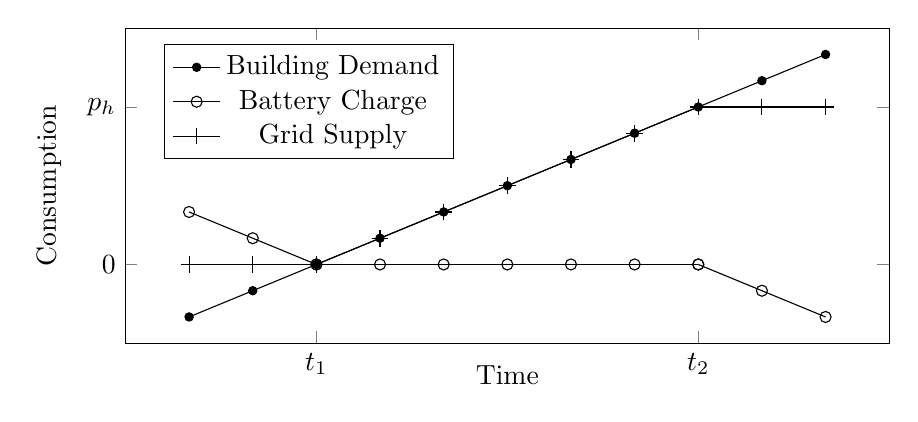
\begin{tikzpicture}

\begin{axis}[
width=0.8\columnwidth,height=4cm,scale only axis,
axis line style={-}, xtick style={-}, ytick style={-},
xlabel=Time,
ylabel=Consumption,
every axis y label/.style={at={(-0.1,0.5)},rotate=90,anchor=center}, 
every axis x label/.style={at={(0.5,-0.1)},anchor=center}, 
%grid=both, grid style={style=densely dotted},
xtick={2,8},
xticklabels={$t_1$,$t_2$},
ytick={0,6},
yticklabels={$0$,$p_h$},
legend style={at={(0.05,0.95)},anchor=north west}
] 

% Draw the Demand-Supply curve
\addplot[-,mark=*,mark size=1.5] expression[domain=0:10,samples=11] {x-2};
\addlegendentry{Building Demand} 

% Draw the Battery curve
\addplot[-,mark=o,mark size=2] expression[forget plot,domain=0:2,samples=3] {2-x}; 
\addplot[-,mark=o,mark size=2] expression[forget plot,domain=2:8,samples=7] {0}; 
\addplot[-,mark=o,mark size=2] expression[domain=8:10,samples=3] {8-x}; 
\addlegendentry{Battery Charge} 

% Draw the Grid supply curve
\addplot[-,mark=+,mark size=3] expression[forget plot,domain=0:2,samples=3] {0}; 
\addplot[-,mark=+,mark size=3] expression[forget plot,domain=2:8,samples=7] {x-2}; 
\addplot[-,mark=+,mark size=3] expression[domain=8:10,samples=3] {6}; 
\addlegendentry{Grid Supply} 
\end{axis} 
\end{tikzpicture} 

%}
}
\qquad
\subfigure[Goal-plan hierarchy for a $k$-modules battery system.]{\label{fig:gptree}
%\resizebox{0.9\columnwidth}{!}{
%!TEX root = ../aamas11storage.tex
\begin{tikzpicture} [level distance=8.0em]
\tikzstyle{planbox}=[draw,text width=11.0em,rectangle split,rectangle split parts=3]
\tikzstyle{goalbox}=[draw,rounded corners=1.25em,minimum height=3em,minimum width=5em]

	
\tikzstyle{level 1}=[sibling distance=13.0em] 
\tikzstyle{level 2}=[level distance=7.0em] 

\node[goalbox,solid] {$G($r,k,s$)$}
	child {node[planbox] {$SetCharge$ 
			\nodepart{second} $\psi:satisfies(r,k,s,C),$\\$k>0$
			\nodepart{third} $set(k,C)$
		}
		child {node[goalbox] {$G($r,k-1,s'$)$}}
	}
	child {node[planbox] {$SetDischarge$ \nodepart{second}
			\nodepart{second} $\psi:satisfies(r,k,s,D),$\\$k>0$
			\nodepart{third} $set(k,D)$
		}
		child {node[goalbox] {$G($r,k-1,s'$)$}}
	}
	child {node[planbox] {$SetNotUsed$ \nodepart{second}
			\nodepart{second} $\psi:satisfies(r,k,s,N),$\\$k>0$
			\nodepart{third} $set(k,N)$
		}
		child {node[goalbox] {$G($r,k-1,s'$)$}}
	}
	child {node[planbox] {$Execute$ 
			\nodepart{second} $\psi:k==0$
			\nodepart{third} $operate()$ \\$evaluate()$
		}
	}
;

\end{tikzpicture}



%}
}
\caption{An energy storage application.}
\end{center}
\label{fig:energystorage}
\end{figure*}


% \newcommand{\aSet}{\mathname{set}}
% \newcommand{\aOperate}{\mathname{operate}}
% \newcommand{\aEvaluate}{\mathname{evaluate}}
% 
% \newcommand{\pSet}{\mathname{Set*}}
% \newcommand{\pSetCharge}{\mathname{SetCharge}}
% \newcommand{\pSetDischarge}{\mathname{SetDischarge}}
% \newcommand{\pSetNotUsed}{\mathname{SetNotUsed}}
% \newcommand{\pExecute}{\mathname{Execute}}
% 
% \newcommand{\cSatisfies}{\psi}
% 
% \begin{figure*}[t]
% \begin{center}
% \subfigure[Use case scenario for a modular battery system.]{\label{fig:usecase}
% %\resizebox{0.9\columnwidth}{!}{
% %!TEX root = ../aamas11storage.tex
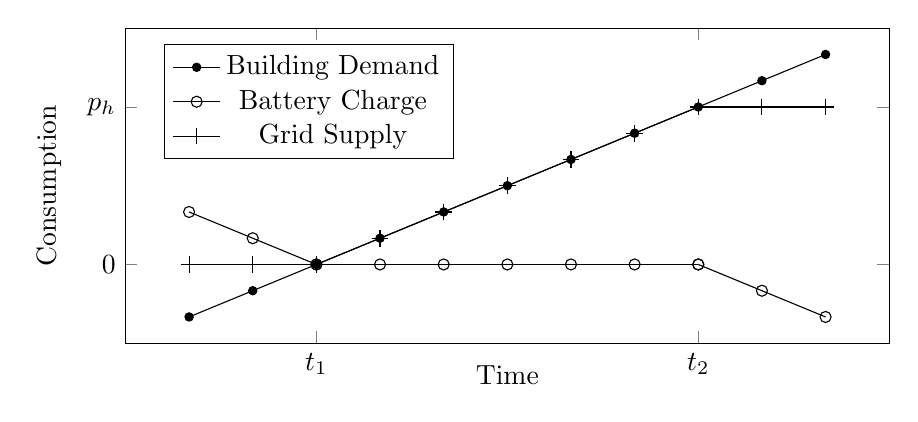
\begin{tikzpicture}

\begin{axis}[
width=0.8\columnwidth,height=4cm,scale only axis,
axis line style={-}, xtick style={-}, ytick style={-},
xlabel=Time,
ylabel=Consumption,
every axis y label/.style={at={(-0.1,0.5)},rotate=90,anchor=center}, 
every axis x label/.style={at={(0.5,-0.1)},anchor=center}, 
%grid=both, grid style={style=densely dotted},
xtick={2,8},
xticklabels={$t_1$,$t_2$},
ytick={0,6},
yticklabels={$0$,$p_h$},
legend style={at={(0.05,0.95)},anchor=north west}
] 

% Draw the Demand-Supply curve
\addplot[-,mark=*,mark size=1.5] expression[domain=0:10,samples=11] {x-2};
\addlegendentry{Building Demand} 

% Draw the Battery curve
\addplot[-,mark=o,mark size=2] expression[forget plot,domain=0:2,samples=3] {2-x}; 
\addplot[-,mark=o,mark size=2] expression[forget plot,domain=2:8,samples=7] {0}; 
\addplot[-,mark=o,mark size=2] expression[domain=8:10,samples=3] {8-x}; 
\addlegendentry{Battery Charge} 

% Draw the Grid supply curve
\addplot[-,mark=+,mark size=3] expression[forget plot,domain=0:2,samples=3] {0}; 
\addplot[-,mark=+,mark size=3] expression[forget plot,domain=2:8,samples=7] {x-2}; 
\addplot[-,mark=+,mark size=3] expression[domain=8:10,samples=3] {6}; 
\addlegendentry{Grid Supply} 
\end{axis} 
\end{tikzpicture} 

% %}
% }
% \qquad
% \subfigure[Goal-plan hierarchy for a $k$-modules battery system.]{\label{fig:gptree}
% %\resizebox{0.9\columnwidth}{!}{
% %!TEX root = ../aamas11storage.tex
\begin{tikzpicture} [level distance=8.0em]
\tikzstyle{planbox}=[draw,text width=11.0em,rectangle split,rectangle split parts=3]
\tikzstyle{goalbox}=[draw,rounded corners=1.25em,minimum height=3em,minimum width=5em]

	
\tikzstyle{level 1}=[sibling distance=13.0em] 
\tikzstyle{level 2}=[level distance=7.0em] 

\node[goalbox,solid] {$G($r,k,s$)$}
	child {node[planbox] {$SetCharge$ 
			\nodepart{second} $\psi:satisfies(r,k,s,C),$\\$k>0$
			\nodepart{third} $set(k,C)$
		}
		child {node[goalbox] {$G($r,k-1,s'$)$}}
	}
	child {node[planbox] {$SetDischarge$ \nodepart{second}
			\nodepart{second} $\psi:satisfies(r,k,s,D),$\\$k>0$
			\nodepart{third} $set(k,D)$
		}
		child {node[goalbox] {$G($r,k-1,s'$)$}}
	}
	child {node[planbox] {$SetNotUsed$ \nodepart{second}
			\nodepart{second} $\psi:satisfies(r,k,s,N),$\\$k>0$
			\nodepart{third} $set(k,N)$
		}
		child {node[goalbox] {$G($r,k-1,s'$)$}}
	}
	child {node[planbox] {$Execute$ 
			\nodepart{second} $\psi:k==0$
			\nodepart{third} $operate()$ \\$evaluate()$
		}
	}
;

\end{tikzpicture}



% %}
% }
% \caption{An energy storage application.}
% \end{center}
% \label{fig:energystorage}
% \end{figure*}


The confidence measure $\C_s$ would make a useful heuristic for exploration (i.e., plan selection) in its own right: such that when the confidence is at its lowest we do maximum exploration and when it is at its highest we fully utilise the decision tree. The problem with this approach, however, is that $\C_s$ only covers the space of known worlds. This means that whenever a new world is witnessed, $\C_s=0.0$, meaning that we will choose randomly. This is hardly beneficial since what we would really like is to use the learnt generalisations to classify this new world rather than be agnostic about it. What is missing is a metric that contributes to our net confidence but that is independent of $w$.

One way to achieve this is by monitoring the rate at which new worlds are being witnessed by the plan $P$. During early exploration it is expected that the majority of worlds that a plan is selected for will be unique, therefore this rate is high and our confidence is low. Over time as exploration continues, the plan would get selected in all possible worlds and the rate of new worlds would approach zero while our confidence over this period would increase to its maximum.  Equation \ref{eqn:confidence-domain} defines this confidence metric $\C_d$ for plan $P$ over the last $n$ executions. Here, $W(P,*)$ is the set of all worlds witnessed by $P$ since the beginning and $\triangle W(P,n)$ is the set of worlds witnessed in the last $n$ executions. $\C_d$ is guaranteed to converge to $1.0$ as long as all worlds where the plan might apply are eventually witnessed.

\begin{equation}
\C_d(P,n) = \frac{|W(P,*)\cap \triangle W(P,n) |}{n}.
\label{eqn:confidence-domain}
\end{equation}

We are now ready to define our final confidence measure $\C$ based on the two component confidence metrics $\C_s$ and $\C_d$. Equation \ref{eqn:confidence} describes this calculation. Here $\alpha$ is the weighting factor used to set a preference bias between the two components.

\begin{equation}
\C(P,w,n) = (\C_s(P,w,n)*\alpha) + [\C_d(P,n)*(1.0-\alpha)].
\label{eqn:confidence}
\end{equation}

Finally, Equation \ref{eqn:omega} shows how the confidence measure $\C$ is used as a exploration heuristic during plan selection. Here $\P$ is the probability of success of plan $P$ in world $w$ as given by its decision tree and $\Omega$ is the plan selection weight. This formulation of the plan selection weight is similar to those presented in \cite{singh10:extending, singh10:learning} bar the replacement of earlier measures with the new confidence term $\C$.

\begin{equation}
\Omega(P,w,n) = 0.5 + \left[  \C(P,w,n) *  \left( \P(P,w) - 0.5 \right)  \right]
\label{eqn:omega}   
\end{equation}

The storage domain scenario (c.f. Section \ref{sec:application}) highlights the benefits of our dynamic confidence measure of Equation \ref{eqn:confidence}. In this domain it is easy to think of situations where the dynamics of the environment changes such that the solution space varies over time. For instance, our motivation for learning is that battery chemistry (and therefore performance) deteriorates over time, and the system should learn to avoid solutions that no longer work in the future. However, worn battery modules get replaced every now and then, and hence, some configurations that the learner may have eliminated previously may become applicable once again. Similar examples may be conjured for situations involving module malfunctions. The point is that each such change in the environment impacts the solution space in some way, however an \notem{signal?} explicit signal is always available to notify us of these changes (some changes may be continuous, for instance). Moreover, several such factors may play on the solution space at one time, and it is up to the learner to respond in this environment appropriately.



Here it becomes important for an agent to reliably recognise such changes, and respond by adjusting its exploration strategy accordingly (or perhaps, switching policies, choosing to learn afresh, and so on). Since the new confidence measure is built using observed data alone, it consequently reflects agent performance: our confidence is maximum when the rate of change in observed performance and worlds states is stable, and minimum when it is not. Importantly, this means that the measure is non-monotonic and as such may be used to dynamically tune the exploration strategy (for instance during plan selection as in Equation \ref{eqn:omega}) against a variable solution space.
